\chapter{Background}

This section presents a block diagram of a proof-of-concept system and introduces many of the concepts and motivations involved in understanding each block.

\section{Field-Programmable Gate Arrays}

\subsection{Architecture}
Inside, an \gls{fpga} consists of a tiled array of interconnected, configurable logic blocks referred to as 'slices', bordered by a series of input / output blocks on the periphery of the device. Inside each slice are a number of fixed resources such as adders, multipliers, registers, \glspl{lut} and memory which can be selectively enabled or disabled to provide reconfigurability. While the number of inputs, outputs and internal resources of a slice varies between \glspl{fpga}, the principle is still the same: use lots of very basic but highly configurable slices to implement any arbitrary digital design. Table \ref{table:clb_resources} shows the resources inside a logic block in the Zynq-7000 \gls{fpga} used for this proof-of-concept.

\begin{table}
    \begin{tabular}{llllll}
        Slices  & LUTs  & Flip-flops    & Arithmetic and carry chains   & Distributed RAM   & Shift registers   \\
        2       & 8     & 16            & 2                             & 256 bits          & 128 bits
    \end{tabular}
    \caption{Logic resources in Zynq-7000 logic block (\url{http://www.xilinx.com/support/documentation/user_guides/ug474_7Series_CLB.pdf}).}
    \label{table:clb_resources}
\end{table}

Combinatorial logic can be implemented using a simple lookup table to map every possible combination of inputs to a specific output value. Essentially a complex block of combinatorial logic can be minimised and the resulting truth table is stored in a \gls{lut}. By combining \glspl{lut} with flip-flops, any digital circuit can be reproduced inside a logic slice given it has sufficient resources. Additionally many logic blocks also contain embedded memory (block RAM and distributed RAM) which can be used to implement small ROMs, RAMs and FIFOs.

Each slice is joined together to form the fabric --- a vast array of configurable logic blocks and configurable interconnect matrices. By chaining together multiple logic blocks it is possible to create highly complex designs. Figure \ref{fig:fpga_diagram} illustrates how each of these resources is connected internally to form the fabric inside an \gls{fpga}. 

\begin{figure}
  \centering
  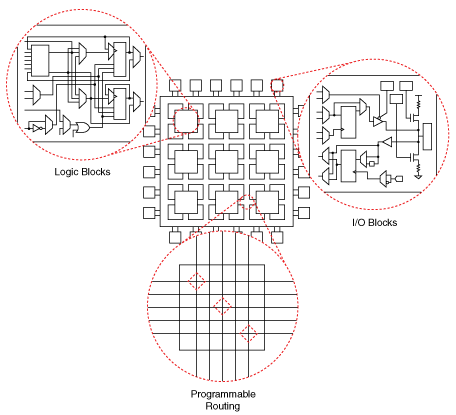
\includegraphics[width=1\textwidth]{./img/fpga_arch_diagram.png}\par
Source: \url{http://zone.ni.com/reference/en-XX/help/371599G-01/lvfpgaconcepts/fpga_basic_chip_terms/}
  \caption{Architectural diagram of \gls{fpga} internals.}
  \label{fig:fpga_diagram}
\end{figure}

\subsection{Hardware Description Languages}
Before \glspl{fpga} became commonplace, custom \glspl{ic} designs were painstakingly designed transistor-by-transistor. The 1970s and 1980s gave away to several \glspl{hdl} --- a new way to formally describe an electronic circuit using a formalised syntax. Fabricating custom \glspl{ic} is a highly complex and expensive process --- designers need to be 100\% certain that the \gls{ic} is sound before taping out the design, or face the huge setbacks (both time and financial) associated with getting it wrong. The abstraction provided by \glspl{hdl} made them very useful for taking an existing design (usually in the form of a captured schematic) and constructing rigorous verification and testing procedures to ensure that the design functions as intended. Despite the test and verification teams being as large, if not larger than the design teams, errors are still made --- most famously an uncaught bug in Intel Pentium processors caused a crash when working with floating-point numbers (\url{http://download.intel.com/support/processors/pentium/sb/FDIV_Floating_Point_Flaw_Pentium_Processor.pdf}). 

Moore's Law saw the transistor counts in \gls{ic} designs grow exponentially to the point where placing individual transistors by hand was no longer feasible. \Glspl{hdl} saw a surge in popularity when they started being used not only for test and verification, but also design. Instead of designing systems at the schematic level, designers used the high-level abstractions that \glspl{hdl} provided to design systems at the \gls{rtl}. Designing at \gls{rtl} level models systems as synchronous digital circuits and required thinking in terms of using hardware registers to store data and the combinatorial logic between them. Designs are typically broken up into individual modules to reduce complexity and increase re-usability, with each module being a isolated set of input and output ports, sequential and combinatorial logic. \Glspl{hdl} are used extensively in modern digital design, with the two most common languages being Verilog (typically favoured in North America) and VHDL (more common in Europe). While modern \glspl{hdl} may resemble common procedural programming languages like C, \glspl{hdl} are fundamentally different in that they describe a concurrent hardware design, rather than a sequentially-executed process. As a result \glspl{fpga} are favoured for problems which benefit from high parallelism and heavy input and output throughput. Verilog was chosen for this project simply because of the author's prior experience with the language.

\subsection{Synthesis and Place-and-Route}

Regardless of whether the target is an \gls{fpga} or a custom \gls{asic}, several additional steps are required to turn a \gls{hdl} design into something which can be run on on the target (or \textit{become} the target in the case of an \gls{asic}). The first step is synthesis, which generates a gate-level schematic for the design. A gate-level representation consists of the design after it is broken down into the most fundamental blocks: flip-flops, latches and combinatorial logic gates.Figure \ref{fig:gate_level} shows the \gls{rtl} representation for the simple Verilog example in Listing \ref{lst:verilog_example}. To infer a registered output, the non-blocking assignment operator \texttt{<=} is used to assign a value to \texttt{Q}. The register input \texttt{D} is assigned the inverted value of output \texttt{Q} using combinatorial logic.

\begin{figure}
  \centering
  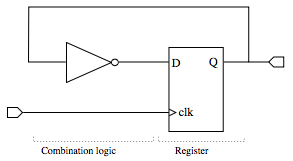
\includegraphics[width=1\textwidth]{./img/gate_level.png}\par
Source: diagram by Alinja, distributed under CC BY-SA 3.0
  \caption{Corresponding gate-level representation of code in Listing \ref{lst:verilog_example}.}
  \label{fig:gate_level}
\end{figure}

\begin{lstlisting}[caption={A basic Verilog example of a register being fed with its own inverted output.}, label={lst:verilog_example}, language=Verilog]
assign D = !Q;

always @(posedge clk) begin
    Q <= D;
end
\end{lstlisting}

Once the design is synthesised it needs to be converted into a format suitable for the target, which is the job of the place-and-route algorithm. The internal architecture of each \gls{fpga} can be very different, and so this process is target-specific. During this process the tools take each part of the gate-level netlist and assign it to a logic block within the \gls{fpga}. After each device has been placed the router will try and determine the optimum way of routing each of the signals between blocks. The place-and-route process is the most critical as it is here where the tools will try and make the design as fast as possible by attempting to optimise any performance-critical which have been constrained by the user with minimum timing requirements specified. Unfortunately it is not always possible to meet these constraints and thus the design may not have the desired performance. One of the most common problems is in trying to route the clock networks so that all devices receive the clock signal at the same time (referred to as clock skew).

\section{CCD and CMOS sensor technologies}

The sensors themselves fall into one of two categories depending on technology used: \gls{ccd} and \gls{cmos}. While both use an array of photosites to collect charge from incident photons during exposure time, the readout and analogue-to-digital conversion process differs for each. During readout time, \glspl{ccd} sequentially shift the accumulated charges into horizontal and vertical readout registers where they are transferred to a chip-level output amplifier and analogue-to-digital converter to generate a binary bitstream. \gls{ccd} image sensors are capable of very low noise and high sensitivity due to the use optimised photosites; this made them a very popular choice for applications demanding high image quality.

Unlike \glspl{ccd}, which rely on a very specialised fabrication process, CMOS sensors can be manufactured using traditional \gls{cmos} processes, benefiting greatly from the associated economies of scale. \gls{aps}, the most common form of \gls{cmos} sensor, differ from \glspl{ccd} in that each photosite contains a dedicated amplifier, meaning that the light-induced voltages can be driven directly to the row and column decoders for digitisation. Because of the \gls{cmos} fabrication process, other camera functions can also be integrated onto the same chip, cutting both the cost and size of the device \cite{10_ge_2012}.  This level of integration, and the faster speeds of parallel readout processing have meant that \gls{cmos} sensors have seen a recent surge in popularity, and are forecast to account for 85\% of the total image sensor market in 2017 \cite{11_ic_insights_2013}.

\begin{figure}
  \centering
  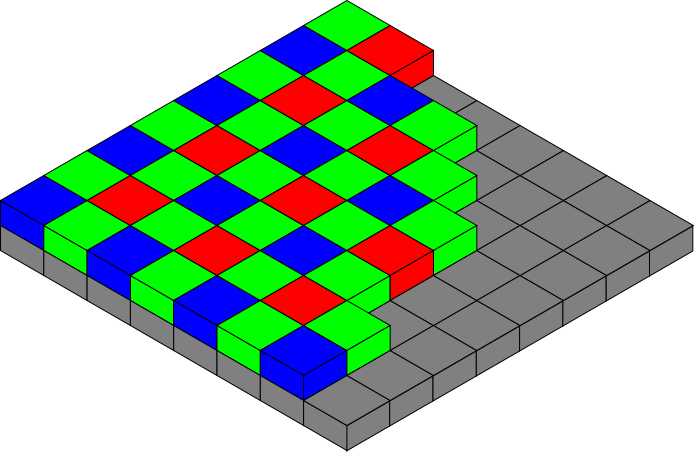
\includegraphics[width=1\textwidth]{./img/bayer_pattern.png}\par
Source: diagram by Cburnett, distributed under CC BY-SA 3.0
  \caption{Bayer filter}
  \label{fig:bayer_pattern}
\end{figure}

Photosites can only measure light intensity, not wavelength, producing greyscale images. By placing a coloured filter in front of each photosite, it is possible to only let light of a certain wavelength through \cite{12_eastman_kodak_company_1976}. Given the fixed pattern of the \gls{cfa}, it is possible to generate a full-colour image using a demosaicing algorithm, the simplest of which is bilinear interpolation, to calculate the red, green and blue intensities for each pixel \cite{13_malvar_he_cutler_2015}. One such \gls{cfa}, the Bayer filter, contains twice as many green elements as red and blue to mimic the physiology of the human eye, as illustrated in Figure \ref{fig:bayer_pattern}.